\documentclass[../main.tex]{subfiles}

\begin{document}

\chapter*{PREFACE}
\label{cha:cha_P_1}
\addcontentsline{toc}{section}{PREFACE}

This book is designed to support a one-semester course in numerical methods. It has been
written for students who want to learn and apply numerical methods in order to solve problems in engineering and science. As such, the methods are motivated by problems rather
than by mathematics. That said, sufficient theory is provided so that students come away
with insight into the techniques and their shortcomings.


$\text{MATLAB}^\copyright$  provides a great environment for such a course. Although other environments (e.g., Excel/VBA, Mathcad) or languages (e.g., Fortran 90, C++) could have
been chosen, MATLAB presently offers a nice combination of handy programming features with powerful built-in numerical capabilities. On the one hand, its M-file programming environment allows students to implement moderately complicated algorithms in a
structured and coherent fashion. On the other hand, its built-in, numerical capabilities
empower students to solve more difficult problems without trying to "reinvent the wheel."


The basic content, organization, and pedagogy of the second edition are essentially
preserved in the third edition. In particular, the conversational writing style is intentionally
maintained in order to make the book easier to read. This book tries to speak directly to the
reader and is designed in part to be a tool for self-teaching.

That said, this edition differs from the past edition in three major ways: (1) two new
chapters, (2) several new sections, and (3) revised homework problems.
\begin{enumerate}
	\item  \textbf{New Chapters.} As shown in \ref{fig:fig_P_1}, I have developed two new chapters for this edition. Their inclusion was primarily motivated by my classroom experience. That is,
they are included because they work well in the undergraduate numerical methods
course I teach at Tufts. The students in that class typically represent all areas of engineering and range from sophomores to seniors with the majority at the junior level. In
addition, we typically draw a few math and science majors. The two new chapters are:
\begin{itemize}
	\item \textbf{Eigenvalues.} When I first developed this book, I considered that eigenvalues might
be deemed an "advanced" topic. I therefore presented the material on this topic at
the end of the semester and covered it in the book as an appendix. This sequencing
had the ancillary advantage that the subject could be partly motivated by the role of
eigenvalues in the solution of linear systems of ODEs. In recent years, I have begun




to move this material up to what I consider to be its more natural mathematical position at the end of the section on linear algebraic equations. By stressing applications (in particular, the use of eigenvalues to study vibrations), I have found that
students respond very positively to the subject in this position. In addition, it allows
me to return to the topic in subsequent chapters which serves to enhance the
students’ appreciation of the topic.
\item  \textbf{Fourier Analysis.} In past years, if time permitted, I also usually presented a lecture
at the end of the semester on Fourier analysis. Over the past two years, I have begun
presenting this material at its more natural position just after the topic of linear least
squares. I motivate the subject matter by using the linear least-squares approach to
fit sinusoids to data. Then, by stressing applications (again vibrations), I have found
that the students readily absorb the topic and appreciate its value in engineering and
science.


It should be noted that both chapters are written in a modular fashion and could
be skipped without detriment to the course's pedagogical arc. Therefore, if you
choose, you can either omit them from your course or perhaps move them to the
end of the semester. In any event, I would not have included them in the current
edition if they did not represent an enhancement within my current experience in
the classroom. In particular, based on my teaching evaluations, I find that the
stronger, more motivated students actually see these topics as highlights. This is
particularly true because MATLAB greatly facilitates their application and interpretation.
\end{itemize}
\item \textbf{New Content.} Beyond the new chapters, I have included new and enhanced sections on a
number of topics. The primary additions include sections on animation (Chap. 3), Brent's
method for root location (Chap. 6), \textsl{LU} factorization with pivoting (Chap. 8), \textsl{random numbers and Monte Carlo simulation} (Chap. 14), \textsl{ adaptive quadrature} (Chap. 20),and \textsl{event termination of ODEs} (Chap. 23).


\item \textbf{New Homework Problems.} Most of the end-of-chapter problems have been modified, and a variety of new problems have been added. In particular, an effort has been
made to include several new problems for each chapter that are more challenging and
difficult than the problems in the previous edition.
\end{enumerate}

\begin{figure}[H]
	\centering
	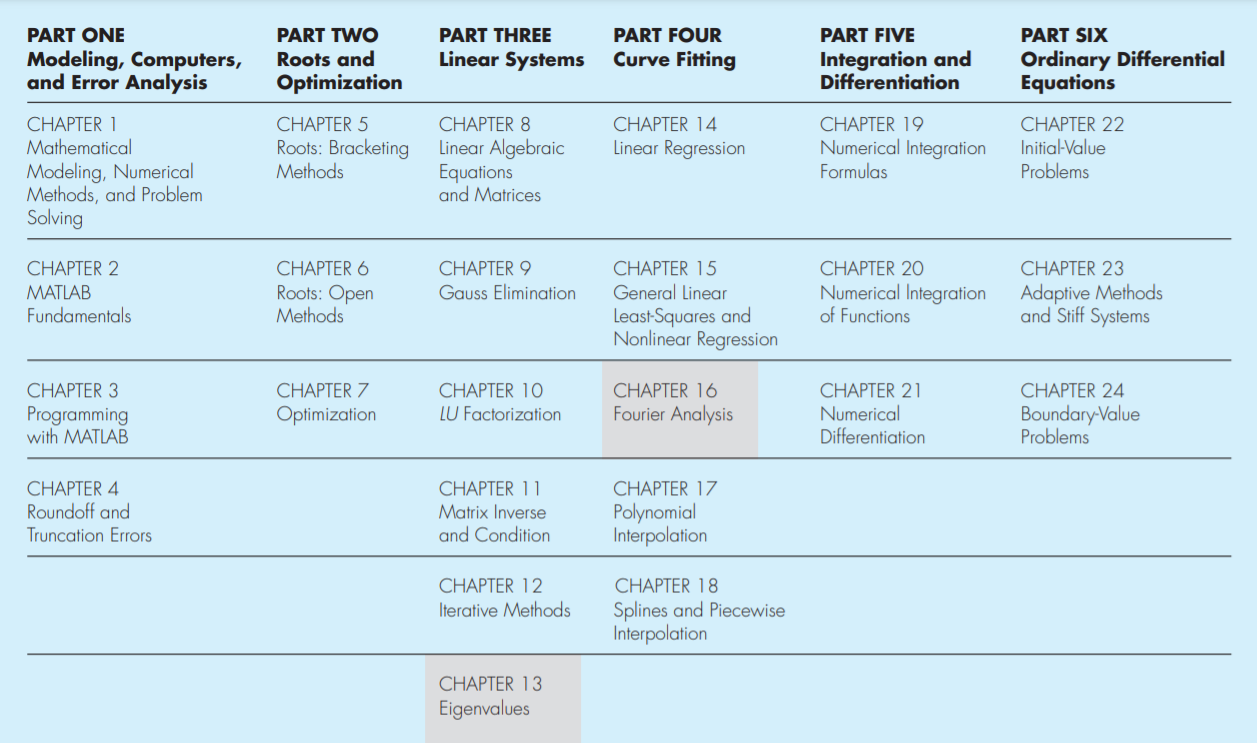
\includegraphics[width=1\linewidth]{fig_P_1.png}
	\caption{\textsf{An outline of this edition. The shaded areas represent new material. In addition, several of the original chapters have been supplemented with
new topics.}}
	\label{fig:fig_P_1}
\end{figure}


Aside from the new material and problems, the third edition is very similar to the second.
In particular, I have endeavored to maintain most of the features contributing to its pedagogical effectiveness including extensive use of worked examples and engineering and scientific applications. As with the previous edition, I have made a concerted effort to make this
book as "student-friendly" as possible. Thus, I’ve tried to keep my explanations straightforward and practical.
Although my primary intent is to empower students by providing them with a sound
introduction to numerical problem solving, I have the ancillary objective of making this
introduction exciting and pleasurable. I believe that motivated students who enjoy engineering and science, problem solving, mathemati cs and yes programming, will ultimately make better professionals. If my book fosters enthusiasm and appreciation for these
subjects, I will consider the effort a success.

\textbf{Acknowledgments}. Several members of the McGraw-Hill team have contributed to
this project. Special thanks are due to Lorraine Buczek, and Bill Stenquist, and Melissa
Leick for their encouragement, support, and direction. Ruma Khurana of MPS Limited, a
Macmillan Company also did an outstanding job in the book’s final production phase. Last,
but not least, Beatrice Sussman once again demonstrated why she is the best copyeditor in
the business.
During the course of this project, the folks at The MathWorks, Inc., have truly demonstrated their overall excellence as well as their strong commitment to engineering and
science education. In particular, Courtney Esposito and Naomi Fernandes of The MathWorks, Inc., Book Program have been especially helpful.
The generosity of the Berger family, and in particular Fred Berger, has provided me
with the opportunity to work on creative projects such as this book dealing with computing
and engineering. In addition, my colleagues in the School of Engineering at Tufts, notably
Masoud Sanayei, Lew Edgers, Vince Manno, Luis Dorfmann, Rob White, Linda Abriola,
and Laurie Baise, have been very supportive and helpful.
Significant suggestions were also given by a number of colleagues. In particular, Dave
Clough (University of Colorado–Boulder), and Mike Gustafson (Duke University) provided valuable ideas and suggestions. In addition, a number of reviewers provided useful
feedback and advice including Karen Dow Ambtman (University of Alberta), Jalal Behzadi
(Shahid Chamran University), Eric Cochran (Iowa State University), Frederic Gibou (University of California at Santa Barbara), Jane Grande-Allen (Rice University), Raphael
Haftka (University of Florida), Scott Hendricks (Virginia Tech University), Ming Huang
(University of San Diego), Oleg Igoshin (Rice University), David Jack (Baylor University), Clare McCabe (Vanderbilt University), Eckart Meiburg (University of California at
Santa Barbara), Luis Ricardez (University of Waterloo), James Rottman (University of
California, San Diego), Bingjing Su (University of Cincinnati), Chin-An Tan (Wayne State
University), Joseph Tipton (The University of Evansville), Marion W. Vance (Arizona
State University), Jonathan Vande Geest (University of Arizona), and Leah J. Walker
(Arkansas State University).
It should be stressed that although I received useful advice from the aforementioned
individuals, I am responsible for any inaccuracies or mistakes you may find in this book.
Please contact me via e-mail if you should detect any errors.
Finally, I want to thank my family, and in particular my wife, Cynthia, for the love,
patience, and support they have provided through the time I’ve spent on this project.
\newpage


\begin{flushright}
Steven C. Chapra\\
Tufts University



Medford, Massachusetts\\
steven.chapra@tufts.edu\\
\end{flushright}


\bigskip
\section*{PEDAGOGICAL TOOLS}
\label{sec:sec_P_1_1}


\textbf{Theory Presented as It Informs Key Concepts.} The text is intended for Numerical Methods users, not developers. Therefore, theory is not included for “theory’s sake,” for example no
proofs. Theory is included as it informs key concepts such as the Taylor series, convergence,
condition, etc. Hence, the student is shown how the theory connects with practical issues in
problem solving.


\textbf{Introductory MATLAB Material.} The text includes two introductory chapters on how to
use MATLAB. Chapter 2 shows students how to perform computations and create graphs
in MATLAB’s standard command mode. Chapter 3 provides a primer on developing
numerical programs via MATLAB M-file functions. Thus, the text provides students with
the means to develop their own numerical algorithms as well as to tap into MATLAB’s
powerful built-in routines.

\textbf{Algorithms Presented Using MATLAB M-files.} Instead of using pseudocode, this book
presents algorithms as well-structured MATLAB M-files. Aside from being useful computer programs, these provide students with models for their own M-files that they will
develop as homework exercises.

\textbf{Worked Examples and Case Studies.} Extensive worked examples are laid out in detail
so that students can clearly follow the steps in each numerical computation. The case studies consist of engineering and science applications which are more complex and richer than
the worked examples. They are placed at the ends of selected chapters with the intention of
(1) illustrating the nuances of the methods, and (2) showing more realistically how the
methods along with MATLAB are applied for problem solving.

\textbf{Problem Sets.} The text includes a wide variety of problems. Many are drawn from engineering and scientific disciplines. Others are used to illustrate numerical techniques and
theoretical concepts. Problems include those that can be solved with a pocket calculator as
well as others that require computer solution with MATLAB.

\textbf{Useful Appendices and Indexes.} Appendix A contains MATLAB commands, and
Appendix B contains M-file functions.

\textbf{Textbook Website.} A text-specific website is available at www.mhhe.com/chapra. Resources include the text images in PowerPoint, M-files, and additional MATLAB resources.
\blankpage




\part{Modeling, Computers,and Error Analysis}
\label{part:part1}

\chapter*{MOTIVATION}
\label{cha:cha1}
What are numerical methods and why should you study them?


\textsl{Numerical methods are techniques by which mathematical problems are formulated so
that they can be solved with arithmetic and logical operations. Because digital computers
excel at performing such operations, numerical methods are sometimes referred to as computer mathematics.}


In the pre–computer era, the time and drudgery of implementing such calculations
seriously limited their practical use. However, with the advent of fast, inexpensive digital
computers, the role of numerical methods in engineering and scientific problem solving
has exploded. Because they figure so prominently in much of our work, I believe that numerical methods should be a part of every engineer’s and scientist’s basic education. Just
as we all must have solid foundations in the other areas of mathematics and science, we
should also have a fundamental understanding of numerical methods. In particular, we should
have a solid appreciation of both their
capabilities and their limitations.
Beyond contributing to your overall
education, there are several additional
reasons why you should study numerical
methods:

\begin{enumerate}
\item Numerical methods greatly expand the
types of problems you can address. They
are capable of handling large systems of
equations, nonlinearities, and complicated geometries that are not uncommon
in engineering and science and that are
often impossible to solve analytically
with standard calculus. As such, they
greatly enhance your problem-solving
skills.
\item Numerical methods allow you to use
“canned” software with insight. During your career, you will invariably have occasion to use commercially available prepackaged computer programs that involve numerical methods. The intelligent use of these
programs is greatly enhanced by an understanding of the basic theory underlying the
methods. In the absence of such understanding, you will be left to treat such packages
as “black boxes” with little critical insight into their inner workings or the validity of
the results they produce.
\item Many problems cannot be approached using canned programs. If you are conversant
with numerical methods, and are adept at computer programming, you can design
your own programs to solve problems without having to buy or commission expensive
software.
\item Numerical methods are an efficient vehicle for learning to use computers. Because numerical methods are expressly designed for computer implementation, they are ideal for
illustrating the computer’s powers and limitations. When you successfully implement
numerical methods on a computer, and then apply them to solve otherwise intractable
problems, you will be provided with a dramatic demonstration of how computers can
serve your professional development. At the same time, you will also learn to acknowledge and control the errors of approximation that are part and parcel of large-scale
numerical calculations.
\item
Numerical methods provide a vehicle for you to reinforce your understanding of mathematics. Because one function of numerical methods is to reduce higher mathematics
to basic arithmetic operations, they get at the “nuts and bolts” of some otherwise
obscure topics. Enhanced understanding and insight can result from this alternative
perspective.
\end{enumerate}

With these reasons as motivation, we can now set out to understand how numerical
methods and digital computers work in tandem to generate reliable solutions to mathematical problems. The remainder of this book is devoted to this task.



\bigskip
\chapter*{ORGANIZATION}
\label{cha:cha2}
This book is divided into six parts. The latter five parts focus on the major areas of numerical methods. Although it might be tempting to jump right into this material, \textsl{Part One} consists of four chapters dealing with essential background material.


\textsl{Chapter 1} provides a concrete example of how a numerical method can be employed
to solve a real problem. To do this, we develop a \textsl{mathematical model} of a free-falling
bungee jumper. The model, which is based on Newton’s second law, results in an ordinary
differential equation. After first using calculus to develop a closed-form solution, we then
show how a comparable solution can be generated with a simple numerical method. We
end the chapter with an overview of the major areas of numerical methods that we cover in
Parts Two through Six.


Chapters 2 and 3 provide an introduction to the $\text{MATLAB}^\copyright$ software environment.
\textsl{Chapter 2} deals with the standard way of operating MATLAB by entering commands one
at a time in the so-called calculator, or command, mode. This interactive mode provides a
straightforward means to orient you to the environment and illustrates how it is used for
common operations such as performing calculations and creating plots.

\textsl{Chapter 3} shows how MATLAB’s programming mode provides a vehicle for assembling individual commands into algorithms. Thus, our intent is to illustrate how MATLAB
serves as a convenient programming environment to develop your own software.


\textsl{Chapter 4} deals with the important topic of error analysis, which must be understood
for the effective use of numerical methods. The first part of the chapter focuses on the
\textsl{roundoff errors} that result because digital computers cannot represent some quantities
exactly. The latter part addresses \textsl{truncation errors} that arise from using an approximation
in place of an exact mathematical procedure.





\blankpage

\chapter{Modeling, Numerical Methods, and Problem Solving}
\pagenumbering{arabic}
\label{cha:cha3}


\begin{center}
\Large{\textbf{CHAPTER OBJECTIVES}}
\end{center}

\normalsize{The primary objective of this chapter is to provide you with a concrete idea of what
numerical methods are and how they relate to engineering and scientific problem
solving. Specific objectives and topics covered are}

\begin{itemize}

\item Learning how mathematical models can be formulated on the basis of scientific

principles to simulate the behavior of a simple physical system.
\item Understanding how numerical methods afford a means to generate solutions in a
manner that can be implemented on a digital computer.

\item Understanding the different types of conservation laws that lie beneath the models
used in the various engineering disciplines and appreciating the difference
between steady-state and dynamic solutions of these models.

\item Learning about the different types of numerical methods we will cover in this
book.

\end{itemize}
\Large{YOU'VE GOT A PROBLEM}


\normalsize{Suppose that a bungee-jumping company hires you. You’re given the task of predicting the velocity of a jumper (Fig. 1.1)  as a function of time during the free-fall part
of the jump. This information will be used as part of a larger analysis to determine the
length and required strength of the bungee cord for jumpers of different mass.
You know from your studies of physics that the acceleration should be equal to the ratio
of the force to the mass (Newton’s second law). Based on this insight and your knowledge of physics and fluid mechanics, you develop the following mathematical model for the rate
of change of velocity with respect to time, }
\newpage

\begin{wrapfigure}{l}{0.25\textwidth}
    \centering
    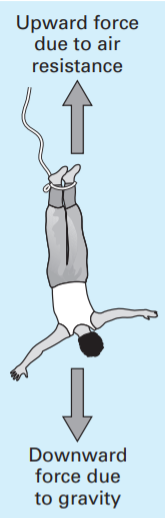
\includegraphics[width=0.25\textwidth]{fig_1_1}
   \caption{\textsf{Forces acting on a free-falling bungee jumper}}
   \label{fig:fig_1_1}
\end{wrapfigure}

$\dfrac{dv}{dt}=g-\dfrac{c_d}{m}v^2$
where $v =$ downward vertical velocity (m/s), $t =$ time (s), $g =$ the acceleration due to
gravity ($\cong$ 9.81 m/s2), $c_d = a$ lumped drag coefficient (kg/m), and $m =$ the jumper’s
mass (kg). The drag coefficient is called “lumped” because its magnitude depends on factors such as the jumper’s area and the fluid density (see Sec 1.4).


Because this is a differential equation, you know that calculus might be used to obtain
an analytical or exact solution for $v$ as a function of $t$. However, in the following pages, we
will illustrate an alternative solution approach. This will involve developing a computeroriented numerical or approximate solution.


Aside from showing you how the computer can be used to solve this particular problem, our more general objective will be to illustrate (a) what numerical methods are and
(b) how they figure in engineering and scientific problem solving. In so doing, we will also
show how mathematical models figure prominently in the way engineers and scientists use
numerical methods in their work.


\bigskip
\section{A SIMPLE MATHEMATICAL MODEL}
\label{sec:sec1}
  A \textsl{mathematical model} can be broadly defined as a formulation or equation that expresses
the essential features of a physical system or process in mathematical terms. In a very general sense, it can be represented as a functional relationship of the form


\begin{equation}
\tag{1.1}
\overset{Dependent}{variable} = f \left( \overset{independent}{variables},parameters,\overset{forcing}{functions}\right)  
\end{equation}
 
where the \textsl{dependent variable} is a characteristic that typically reflects the behavior or state
of the system; the independent variables are usually dimensions, such as time and space,
along which the system’s behavior is being determined; the parameters are reflective of the
system's properties or composition; and the forcing functions are external influences acting
upon it.

The actual mathematical expression of Eq. (1.1) can range from a simple algebraic
relationship to large complicated sets of differential equations. For example, on the basis of
his observations, Newton formulated his second law of motion, which states that the time
rate of change of momentum of a body is equal to the resultant force acting on it. The mathematical expression, or model, of the second law is the well-known equation

\begin{equation}
\tag{1.2}
F=ma
\end{equation}

where $F$ is the net force acting on the body $(N, or kg m/s^2
), m$ is the mass of the object (kg),
and a is its acceleration $(m/s^2
)$.

The second law can be recast in the format of Eq. (1.1) by merely dividing both sides
by $m$ to give
\begin{equation}
\tag{1.3}
a=\dfrac{F}{m}
\end{equation}

where $a$ is the dependent variable reflecting the system's behavior, $F$ is the forcing function, and $m$ is a parameter. Note that for this simple case there is no independent variable
because we are not yet predicting how acceleration varies in time or space.

\begin{itemize}
\item  It describes a natural process or system in mathematical terms.
\item It represents an idealization and simplification of reality. That is, the model ignores negligible details of the natural process and focuses on its essential manifestations. Thus,
the second law does not include the effects of relativity that are of minimal importance
when applied to objects and forces that interact on or about the earth’s surface at velocities and on scales visible to humans.
\item  Finally, it yields reproducible results and, consequently, can be used for predictive purposes. For example, if the force on an object and its mass are known, Eq. (1.3) can be
used to compute acceleration.

\end{itemize}


Because of its simple algebraic form, the solution of Eq. (1.2) was obtained easily.
However, other mathematical models of physical phenomena may be much more complex,
and either cannot be solved exactly or require more sophisticated mathematical techniques
than simple algebra for their solution. To illustrate a more complex model of this kind,
Newton’s second law can be used to determine the terminal velocity of a free-falling body
near the earth’s surface. Our falling body will be a bungee jumper (Fig. 1.1). For this case,
a model can be derived by expressing the acceleration as the time rate of change of the
velocity $(dv/dt)$ and substituting it into Eq. (1.3) to yield

\begin{equation}
\tag{1.4}
\dfrac{dv}{dt}=\dfrac{F}{m}
\end{equation}
where $v$ is velocity (in meters per second). Thus, the rate of change of the velocity is equal
to the net force acting on the body normalized to its mass. If the net force is positive, the
object will accelerate. If it is negative, the object will decelerate. If the net force is zero, the
object's velocity will remain at a constant level.


Next, we will express the net force in terms of measurable variables and parameters.
For a body falling within the vicinity of the earth, the net force is composed of two opposing forces: the downward pull of gravity $F_D$ and the upward force of air resistance $F_U$
(Fig. 1.1):

\begin{equation}
\tag{1.5}
F= F_D + F_U
\end{equation}

If force in the downward direction is assigned a positive sign, the second law can be
used to formulate the force due to gravity as

\begin{equation}
\tag{1.6}
F_D=mg
\end{equation}
where g is the acceleration due to gravity $(9.81 m/s^2
)$.

Air resistance can be formulated in a variety of ways. Knowledge from the science of
fluid mechanics suggests that a good first approximation would be to assume that it is proportional to the square of the velocity,

\begin{equation}
\tag{1.7}
F_U=-c_dv^2
\end{equation}

where $c_d$ is a proportionality constant called the \textsl{lumped drag coefficient} (kg/m). Thus, the
greater the fall velocity, the greater the upward force due to air resistance. The parameter
$c_d$ accounts for properties of the falling object, such as shape or surface roughness, that affect air resistance. For the present case, $c_d$ might be a function of the type of clothing or the
orientation used by the jumper during free fall.
The net force is the difference between the downward and upward force. Therefore,
Eqs. (1.4) through (1.7) can be combined to yield
\begin{equation}
\tag{1.8}
\dfrac{dv}{dt}=g-\dfrac{C_d}{m}v^2
\end{equation}

Equation (1.8) is a model that relates the acceleration of a falling object to the forces
acting on it. It is a \textsl{differential equation} because it is written in terms of the differential rate
of change $(dv/dt)$ of the variable that we are interested in predicting. However, in contrast
to the solution of Newton's second law in Eq. (1.3), the exact solution of Eq. (1.8) for the
velocity of the jumper cannot be obtained using simple algebraic manipulation. Rather,
more advanced techniques such as those of calculus must be applied to obtain an exact or
analytical solution. For example, if the jumper is initially at rest $(v = 0 at t = 0)$, calculus
can be used to solve Eq. (1.8) for

\begin{equation}
\tag{1.9}
v(t)=\sqrt{\dfrac{gm}{c_d}}tanh \left(\sqrt{\dfrac{gc_d}{m}t}\right)
\end{equation}
where tanh is the hyperbolic tangent that can be either computed directly\footnote{{}MATLAB allows direct calculation of the hyperbolic tangent via the built-in function $tanh(x)$.} or via the more
elementary exponential function as in

\begin{equation}
\tag{1.10}
tanhx=\dfrac{e^x-e^{-x}}{e^x+e^{-x}}
\end{equation}

Note that Eq. (1.9) is cast in the general form of Eq. (1.1) where $v(t)$ is the dependent
variable, $t$ is the independent variable, $c_d$ and $m$ are parameters, and $g$ is the forcing function.


\bigskip
\section*{EXAMPLE 1.1. Analytical Solution to the Bungee Jumper Problem }
\label{sec:sec3}
\textbf{Problem Statement.} A bungee jumper with a mass of 68.1 kg leaps from a stationary hot
air balloon. Use Eq. (1.9) to compute velocity for the first 12 s of free fall. Also determine
the terminal velocity that will be attained for an infinitely long cord (or alternatively, the
jumpmaster is having a particularly bad day!). Use a drag coefficient of 0.25 kg/m.

\textbf{Solution.} Inserting the parameters into Eq. (1.9) yields

$$ 
v(t) =\sqrt{\dfrac{9.81(68.1)}{0.25}}tanh \left(\sqrt{\dfrac{9.81(0.25)}{68.1}}t\right)= 51.6938 tanh(0.18977t)
$$
\newpage
which can be used to compute

\begin{figure}[H]
	\centering
	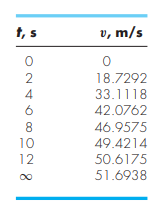
\includegraphics[width=0.25\textwidth]{fig_1_1s}
   \label{fig:fig_1_1s}
\end{figure}



According to the model, the jumper accelerates rapidly (Fig. 1.2). A velocity of
49.4214 m/s (about 110 mi/hr) is attained after 10 s. Note also that after a sufficiently long

\begin{figure}[H]
	\centering
	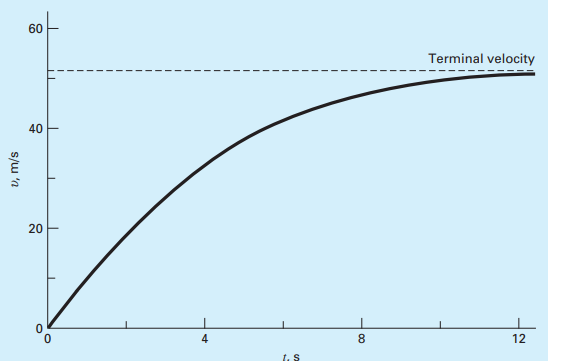
\includegraphics[width=0.75\textwidth]{fig_1_2}
   \caption{\textsf{The analytical solution for the bungee jumper problem as computed in Example 1.1. Velocity
increases with time and asymptotically approaches a terminal velocity.}}
   \label{fig:fig_1_2}
\end{figure}

time, a constant velocity, called the terminal velocity, of 51.6983 m/s (115.6 mi/hr) is
reached. This velocity is constant because, eventually, the force of gravity will be in balance with the air resistance. Thus, the net force is zero and acceleration has ceased.


Equation (1.9) is called an analytical or closed-form solution because it exactly satisfies the original differential equation. Unfortunately, there are many mathematical models
that cannot be solved exactly. In many of these cases, the only alternative is to develop a
numerical solution that approximates the exact solution.
\textit{Numerical methods} are those in which the mathematical problem is reformulated so it
can be solved by arithmetic operations. This can be illustrated for Eq. (1.8) by realizing that
the time rate of change of velocity can be approximated by (Fig. 1.3):

\begin{equation}
\tag{1.11}
\dfrac{dv}{dt}\cong\dfrac{\Delta v}{\Delta t} = \dfrac{v(t_{i+1})-v(t_i)}{t_{i+1}-t_i}
\end{equation}

where $\Delta v$ and $\Delta t$ are differences in velocity and time computed over finite intervals, $v(t_i)$
is velocity at an initial time $t_i$, and $v(t_{i+1})$ is velocity at some later time $(t_{i+1})$. Note that
$dv/dt \cong \Delta v / \Delta t$ is approximate because $ \Delta t$ is finite. Remember from calculus that
$$
\dfrac{dv}{dt} = \lim_{\Delta t\to 0} \dfrac{\Delta v}{ \Delta t}
$$

Equation (1.11) represents the reverse process.

\begin{figure}[H]
	\centering
	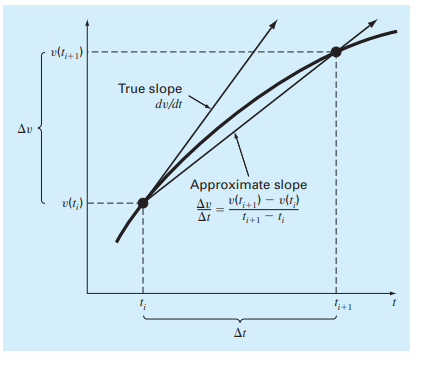
\includegraphics[width=0.75\textwidth]{fig_1_3}
   \caption{\textsf{The use of a finite difference to approximate the first derivative of v with respect to t.}}
   \label{fig:fig_1_3}
\end{figure}


\end{document}